% Options for packages loaded elsewhere
\PassOptionsToPackage{unicode}{hyperref}
\PassOptionsToPackage{hyphens}{url}
%
\documentclass[
]{article}
\usepackage{amsmath,amssymb}
\usepackage{lmodern}
\usepackage{ifxetex,ifluatex}
\ifnum 0\ifxetex 1\fi\ifluatex 1\fi=0 % if pdftex
  \usepackage[T1]{fontenc}
  \usepackage[utf8]{inputenc}
  \usepackage{textcomp} % provide euro and other symbols
\else % if luatex or xetex
  \usepackage{unicode-math}
  \defaultfontfeatures{Scale=MatchLowercase}
  \defaultfontfeatures[\rmfamily]{Ligatures=TeX,Scale=1}
\fi
% Use upquote if available, for straight quotes in verbatim environments
\IfFileExists{upquote.sty}{\usepackage{upquote}}{}
\IfFileExists{microtype.sty}{% use microtype if available
  \usepackage[]{microtype}
  \UseMicrotypeSet[protrusion]{basicmath} % disable protrusion for tt fonts
}{}
\makeatletter
\@ifundefined{KOMAClassName}{% if non-KOMA class
  \IfFileExists{parskip.sty}{%
    \usepackage{parskip}
  }{% else
    \setlength{\parindent}{0pt}
    \setlength{\parskip}{6pt plus 2pt minus 1pt}}
}{% if KOMA class
  \KOMAoptions{parskip=half}}
\makeatother
\usepackage{xcolor}
\IfFileExists{xurl.sty}{\usepackage{xurl}}{} % add URL line breaks if available
\IfFileExists{bookmark.sty}{\usepackage{bookmark}}{\usepackage{hyperref}}
\hypersetup{
  hidelinks,
  pdfcreator={LaTeX via pandoc}}
\urlstyle{same} % disable monospaced font for URLs
\usepackage[margin=1in]{geometry}
\usepackage{longtable,booktabs,array}
\usepackage{calc} % for calculating minipage widths
% Correct order of tables after \paragraph or \subparagraph
\usepackage{etoolbox}
\makeatletter
\patchcmd\longtable{\par}{\if@noskipsec\mbox{}\fi\par}{}{}
\makeatother
% Allow footnotes in longtable head/foot
\IfFileExists{footnotehyper.sty}{\usepackage{footnotehyper}}{\usepackage{footnote}}
\makesavenoteenv{longtable}
\usepackage{graphicx}
\makeatletter
\def\maxwidth{\ifdim\Gin@nat@width>\linewidth\linewidth\else\Gin@nat@width\fi}
\def\maxheight{\ifdim\Gin@nat@height>\textheight\textheight\else\Gin@nat@height\fi}
\makeatother
% Scale images if necessary, so that they will not overflow the page
% margins by default, and it is still possible to overwrite the defaults
% using explicit options in \includegraphics[width, height, ...]{}
\setkeys{Gin}{width=\maxwidth,height=\maxheight,keepaspectratio}
% Set default figure placement to htbp
\makeatletter
\def\fps@figure{htbp}
\makeatother
\setlength{\emergencystretch}{3em} % prevent overfull lines
\providecommand{\tightlist}{%
  \setlength{\itemsep}{0pt}\setlength{\parskip}{0pt}}
\setcounter{secnumdepth}{-\maxdimen} % remove section numbering
\ifluatex
  \usepackage{selnolig}  % disable illegal ligatures
\fi

\author{}
\date{\vspace{-2.5em}}

\begin{document}

\section{Casein and its interaction properties in complex food systems}

In many complex, highly concentrated food systems, characteristic
structure-forming processes take place that have so far only been
described in phenomenological terms. The structure of food products is
created during the process of transforming the raw materials into the
final product (@McClements). Overall, it shapes the mouthfeel, which is
expressed via sensory attributes such as creaminess, etc., but also
plays a role in determining the intensity of the taste and aroma
sensation.

The dominant structure-forming components are mostly proteins that are
ready to aggregate. Protein-rich product systems play an increasingly
important role in human nutrition, but also in pharmaceutical
biotechnology. Examples are clinical and geriatric nutrition, where
swallowing problems require a specific structure or viscosity
controllable by protein aggregates, e.g.~to circumvent the problem of
``dysphagia''. On the other hand, in certain neurodegenerative
phenomena, the occurrence of chronic diseases is often associated with
the phenomenon of aggregation, albeit under very different milieu
conditions than in food, as it was reported in @Mezzenga2013.

Elderly people and athletes require protein-rich foods to counteract
progressive muscle loss and to support muscle building, respectively.
Ignorant of the fundamental interrelationships of the structure-forming
potential of proteins in highly concentrated systems, especially in
complex multi-phased systems, one is currently not yet sufficiently able
to make targeted use of protein-based structure formation in the sense
of efficient, quality- and productivity-guided process control. Further,
many modern pharmaceuticals today are proteins whose aggregation
behavior determines their efficacy as therapeutic agents.

An emerging trend is the need for structure formation by rapid
aggregation, generally for intensification (i.e excelaration or yield
increase) of processes or, for example, in the design of food products
in 3D printing processes. Here, novel structure formation processes are
a prerequisite to achieve spontaneous solidification of the structure
built from liquid or pasty base materials. As a recent example for this
emerging trend, the work of @Kang2021 describes 3D printing of cultured
meat cells derived from stem-cells into structures similar to fresh-cut
meat from Waygu beef. The procedure hereby consisted of printing fibres
from muscle and adipose tissue into a tendon-gel, which serves as the
meat matrix. Accordingly, the formation of the gel in which novel food
structures can be incorporated as well as the pronting process itself
are of interest when it comes to aggregation phenomena in food systems.

In order to target such specific structure formation processes, it is
necessary to understand protein aggregation and especially the
interaction with dispersed phases on a molecular level (@Hubbard2003a,
@McClements). Many studies have been performed on a microscopic scale on
the aggregation phenomena in colloidal, or rather liquid systems such as
emulsions made from caseins (@Brunner1991, @Alexander2006, @Mizuno2005,
@Liang2013 ,@WONG201291). On the other side of the spectrum, many
studies have been performed on the physical properties of gelled or
solidified systems (@Matsumura1993a, @Brighenti2018, @Berta2016,
@Sadlikova2010, @Salek2017).

If one wanted to analyze both effects simultaniously, i.e.~the effects
coming from a proteinogenic phase interacting with a dispersed phase, as
well as the effects of gelation of said proteins, a system must be
investigated, that shows both properties. The gain of knowledge coming
from the investigation of such systems would be, that further insight
could be given as to how a dispersed phase either stabilizes or
destabilizes such systems, and if the formation of a continous network
is overall influenced by the presence of a dispersed phase.

A specific food system, which can be generalized in a way that it is
generic towards many food systems, is processed or cream cheese. On the
one hand, it is a heat-set gel, where aggregation processes occur during
the heating phase, that lead to a gelled structure in cold state. On the
other hand, it has a dispersed phase embedded in the gel structure,
wherein the emulsification of the dispersed phase also occurs during the
heating phase. The heating phase is referred to as processing, however
the term processed cheese should not lead to the assumption that
store-type cream cheese is processed without the use of heat. An
intensive study on the structural behaviour of commercial cream-cheese
products has been performed by @Dang2019. Structure formation processes
in processed, or sometimes also referred to as analogue cheese samples
was investigated extensively also in recent years, Tablexx gives a non
conclusive overview of studies performed in such systems.

@Lamichhane2018 gave an overview for the scale levels in native cheese
and their functional domains. On the molecular scale, milk salts,
lactose, water and whey proteins can be found. The nano-scale which
presents to be an important scale for the formation of complex
structures, casein aggregates and on the higher nano scale casein
micelles can be found. The micro scale in processed cheese is manly
attributed to emulsified fat-globules or fat-particles. Native fat
globules are not to be found in processed cheese models that are not
using dairy cream as the fatty or dispersed phase. The macroscale
represents the scale visible to the human eye and represents visible
chrystals or cracks in the structure.

\begin{figure}
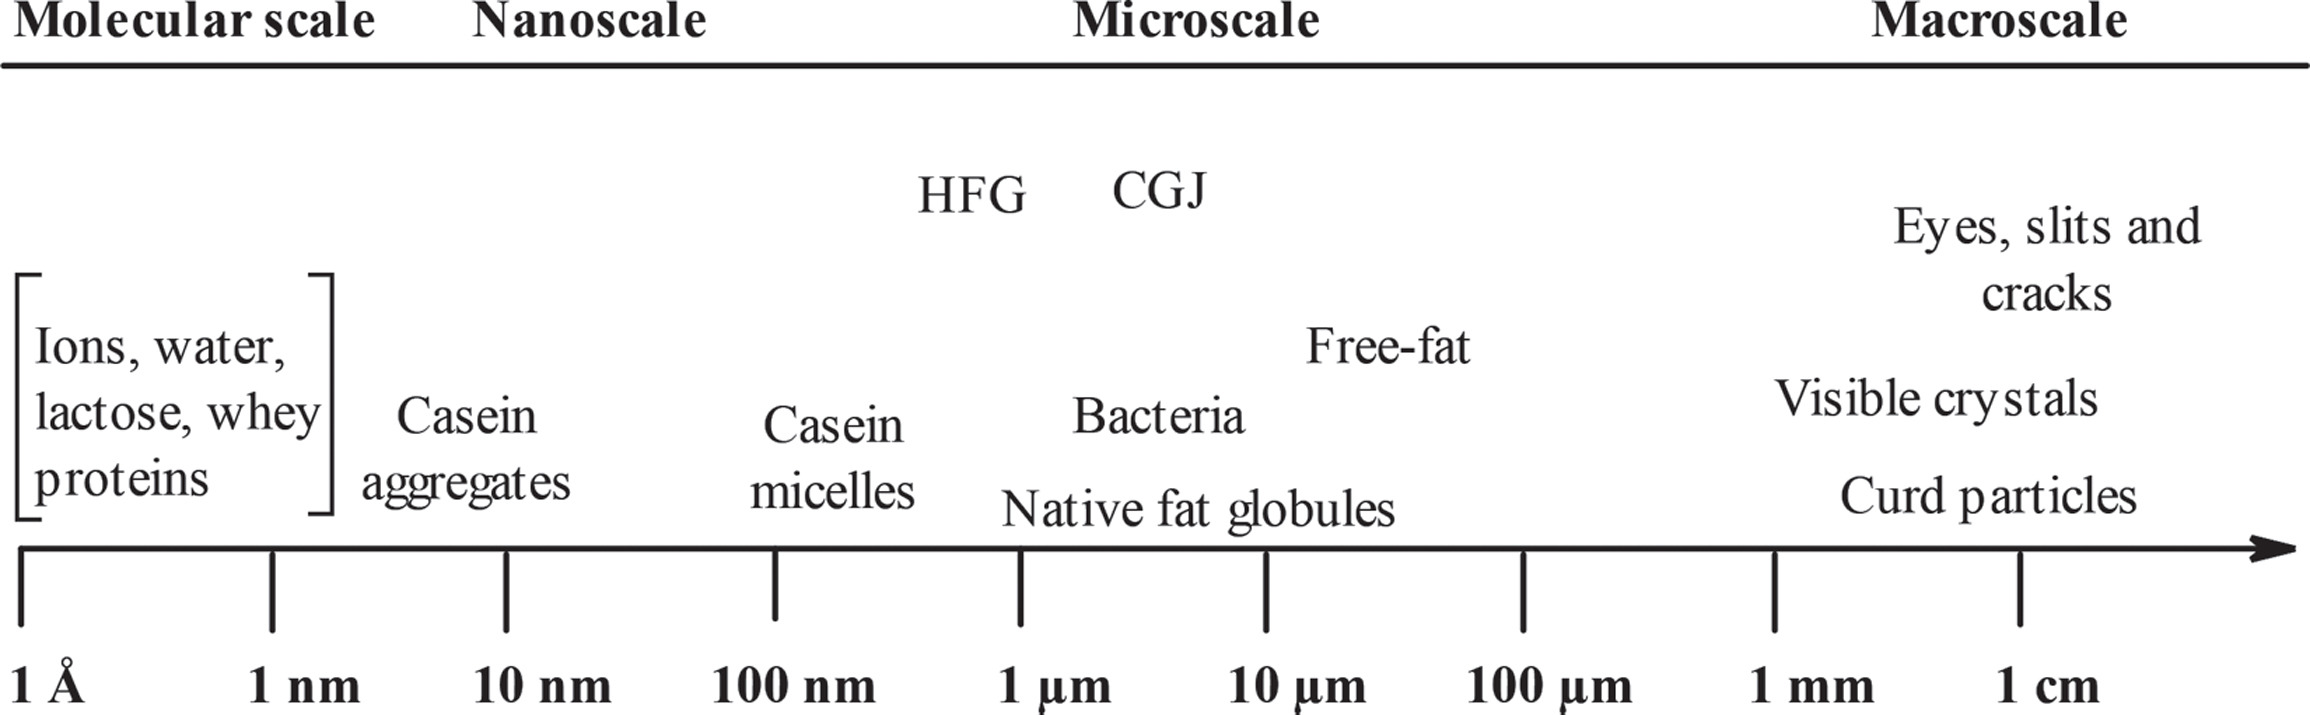
\includegraphics[width=0.75\linewidth]{images/scales_cheese_Lamichhane2018} \caption{Structures found in cheese in the micro-, meso-, and macroscale [@Lamichhane2018] }\label{fig:unnamed-chunk-1}
\end{figure}

Such systems can be considered as emusion gels or `soft-solids', as in
@Dickinson2012a, where they are either characterized as an emulsion
filled or particulate gel. Hence the main difference lies in the
embedding of the dispersed phase into the structured continous phase.

The structured continous phase in processed or cream cheese is built by
caseins. As amphoteric proteins, caseins also emulsify the fat or fatty
phase. Hence, investigating processed or cream cheese as a
representative for a soft, solidified or gelled dispersed food system
can provide insight into the structuring mechanisms of such structures.
It might also give hints towards the occurence of aggregation phenomena,
or investigations of such, in biogenic systems in general. This concept
is explored further down below.

\subsection{Casein: structure and functionality}

Milk contains two main classes of proteins, the mostly globular and heat
sensitive whey proteins and the major milk proteins: caseins. Caseins
can be isolated from milk, using acid treatment at pH 4.6 and 20°C.
Under these circumstances, the Caseins will percipitate due to the
screening of electrostatic repulsion. This happens as an effect of being
close to the IEP, whereas whey (and other) proteins will stay in
solution. Calcium percipitation of caseins can be also used in a
targeted manner, to isolate specific caseins from the micelle by their
differences in calcium sensitivity (@Post2012). Since milk proteins are
thus seperated relatively easy, first research on Caseins was performed
as early as the beginning of the 19th century (@Huppertz2018a).

The Casein Micelle is a highly aggregated particle, stabilized by
hydrophobic interactions and electrostatic interactions internally.
Externally, it is stabilized by steric repulsion through the outer
``hairy-layer'', mainly consisting of kappa casein. With a surface area
of about 4000 m2/l at a specific mass of 1.11 g/ml (20°C) and a number
of 1014-1016 micelles/ml of raw milk, caseins are the main component of
milk proteins. This is also represented by the strong hydration
properties of the casein micelle. Caseins are reported to display a mean
hydrodynamic radius within a range of 50-500 nm and are able to bind up
to 2.5 g of water per gram protein. Thus, caseins make up
\textasciitilde13\% of the volume fraction of milk, roughly five times
higher than their dehydrated mass proportion in milk (@Dalgleish2012,
@Fox2009).

The average molecular weight of a dehydrated micelle is about 108
daltons. The micelle itself is composed of four different casein
fractions, of which different genetic variants exist: alphaS1-,
alphaS2-, beta- and kappa-casein. The percentage ratio of the total
protein is 30:8:30:10. The dry matter of a micelle comprises 94\%
protein and 6\% colloidal calcium phosphate (CCP). CCP further comprises
magnesium, calcium, phosphate, citrate, sodium and potassium ions
(@Gaucheron2012). The exact structure of the casein micelle is not yet
fully known and many models have been proposed, most recently by
@Dalgleish2012.

The effect of high pressure (150-300MPa) on the casein micelle structure
in milk showed the occurence of small micelles next to large micelles
under the use of cryo-transmission electron microscopy (cryo-TEM).
Higher pressurization rates of 400 MPa resulted in the formation of
smaller casein assemblies of 30-100 nm in size. It was also found, that
free Calcium was taken in by the casein structures and that the
substructures induced by high pressure treatment can be also found in
untreated milk (@Knudsen2010). This shows, that the caseins are highly
prone to self-assembly and aggregation, especially under the presence of
calcium ions.

To this day, the inner structure of the casein micelle is unclear.
Elucidation of the inner structure using imaging techniques such as
transmission electron microscopy (TEM) is not possible, since the
molecular density in the casein micelle is too high. The sub micelle
binding model, presented by @WALSTRA1999189 but developed from
preceeding models considers the casein micelle to be an aggregated
particle made out of, again micellar substructures. In the sub-micelles
the CCP is incorporated. On the surface of the casein micelle, a
so-called ``hairy-layer'' made out of kappa casein prevents the micelles
from \emph{in-situ} aggregation in milk, due to steric and elctrostatic
repulsion. This model is grounded on experimental evidence. It was, for
example, shown that casein monomers self-assemble into sub-micelles,
when calcium ions are present.

\begin{figure}
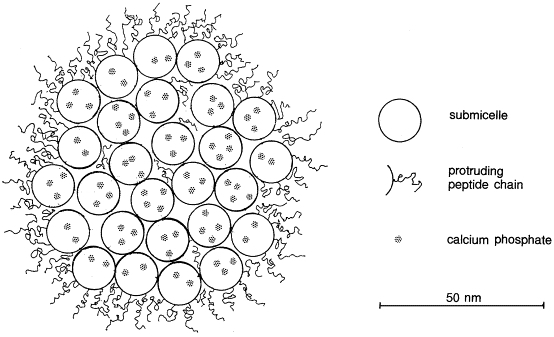
\includegraphics[width=0.5\linewidth]{images/micelle_Walstra} \caption{Sub-micelle binding model as presented by @WALSTRA1999189: caseins are arranged in spherical sub-micelles, in which CCPs are incorporated}\label{fig:unnamed-chunk-2}
\end{figure}

In later models, the focus of casein micelle stabilization was shifted
to the calcium phosphate nano-clusters (CCP). The nano cluster model
(Holt et al.~(1998)) was followed by the dual binding model. Both models
suspected the CCP to stabilize the casein micelle internally, as well as
hydrophobic interactions in balance with electrostatic repulsion.

According to investigations of @Huppertz2017, the stabilisation of the
micelle in the interior takes place via the CCP nano-clusters. This was
found by investigating differently bound water in the casein micelle. It
was possible to identify non-sperical particles, which were referred to
as primary casein particles (PCP), which form a porous micelle structure
through linkages via calcium phosphate nanoclusters. What's interesting
here is that seemingly rebuilt casein micelles from sodium caseinate
displayed similar properties as native and dried casein micelles in
terms of radius of gyration, or particle size.

\begin{figure}
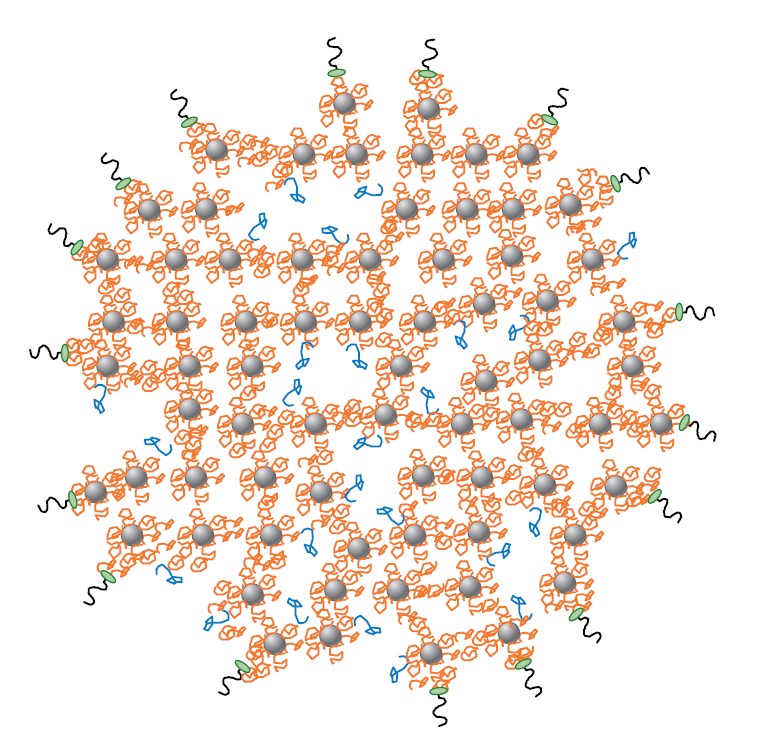
\includegraphics[width=0.5\linewidth]{images/micelle_Dalgleish} \caption{Dual-Binding model of the casein micelle by @Dalgleish2012a: beta and alpha-caseins (orange) are connected to the CCP(grey spheres); blue represents free beta-casein, hydrophobically bound. Micelle is stabilized by k-casein (green) wherein the black coil represents the Casein Macropeptide (CMP) }\label{fig:unnamed-chunk-3}
\end{figure}

In the model of the casein micelle from @Dalgleish2012a, CCPs are
connected to the phosphorylated serine side chains of the caseins via a
calcium phosphate bridge, as indicated by the grey spheres. Furthermore,
hydrophobic interactions and van der Waals forces contribute to the
stabilisation. Among the casein fractions homogeneously distributed
inside, the kappa casein sits at the surface of the micelle and
stabilises the micelle through its outwardly directed, strongly
hydrophilic and negatively charged part, the casein macropeptide (CMP).
The negative charge causes steric repulsion of the micelles from each
other, which leads to colloidal stability of the micelle. The hydrate
shell additionally stabilises the micelle. The kappa casein as
``hairy-layer'' is also presented in the dual binding model. Also of
importance is the fact that a casein micelle is not a static system, but
is in a dynamic equilibrium with the milk serum. This equilibrium can be
disturbed mainly due to the calcium sensitivity of the individual casein
fractions. While kappa-casein reacts quite insensitively to calcium
ions, the two alphaS-fractions are strongly calcium-sensitive
(@Holt2013). By binding calcium ions on the surface, the outer
kappa-casein protects the calcium-sensitive casein fractions inside the
micelle and thus prevents a calcium-induced structural change
@Huppertz2018a. An overview of the distribution of the calcium in the
casein micelle was presented in @Dumpler2018 and can be seen in Fig.xx.

\begin{figure}
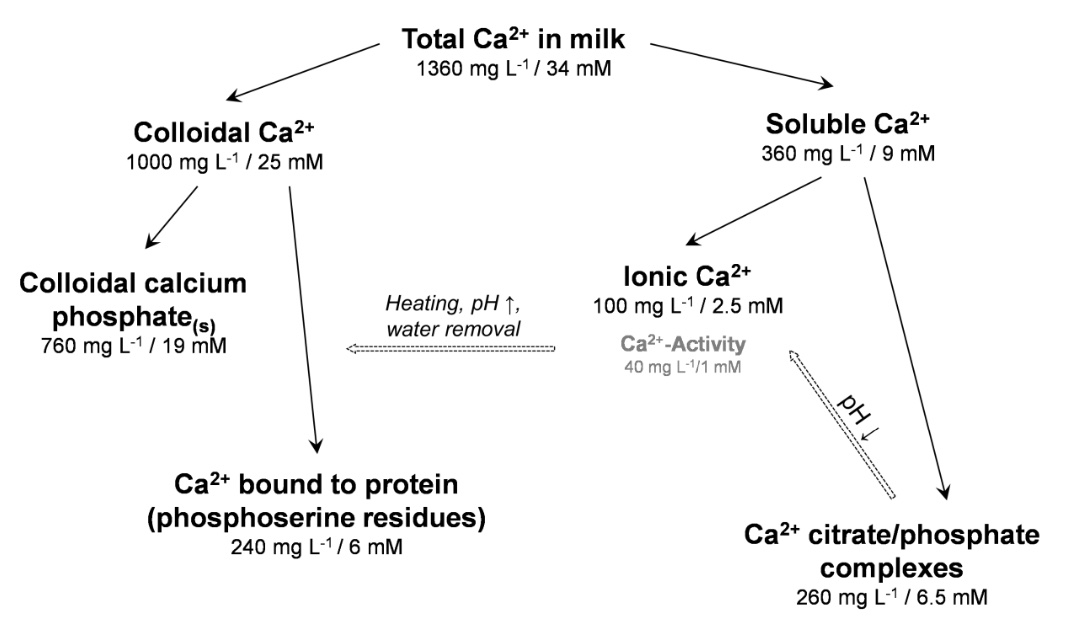
\includegraphics[width=0.75\linewidth]{images/calcium_dumpler} \caption{Distribution of calcium in milk}\label{fig:unnamed-chunk-4}
\end{figure}

From that it can be seen, that the binding state of calcium in the
casein micelle is dependent on milieu conditions (pH, water
concentration, Temperature).

\subsection{Overview of gelation mechanisms}

Gelation of biopolymers is a phenomenon generally recognized as the
solidification of a matrix by interaction(s) of the biopolymers, here
proteins, with the solvent. Gelation can happen due to various reasons,
Fig.xx gives an overview of gelation mechanisms in general. Gelation
induced by the formation of covalent bonds is used often in organic, non
edible gels as in acrylamide gels for gel-electrophoresis. Covalent
gelation in casein occurs, when treated enzymatically with
transgrlutaminase, which connects the glutamine residues in a protein by
intramolecular bonds. In general, gels from casein are particle gels, as
in (D) of Fig.xx.

\begin{figure}
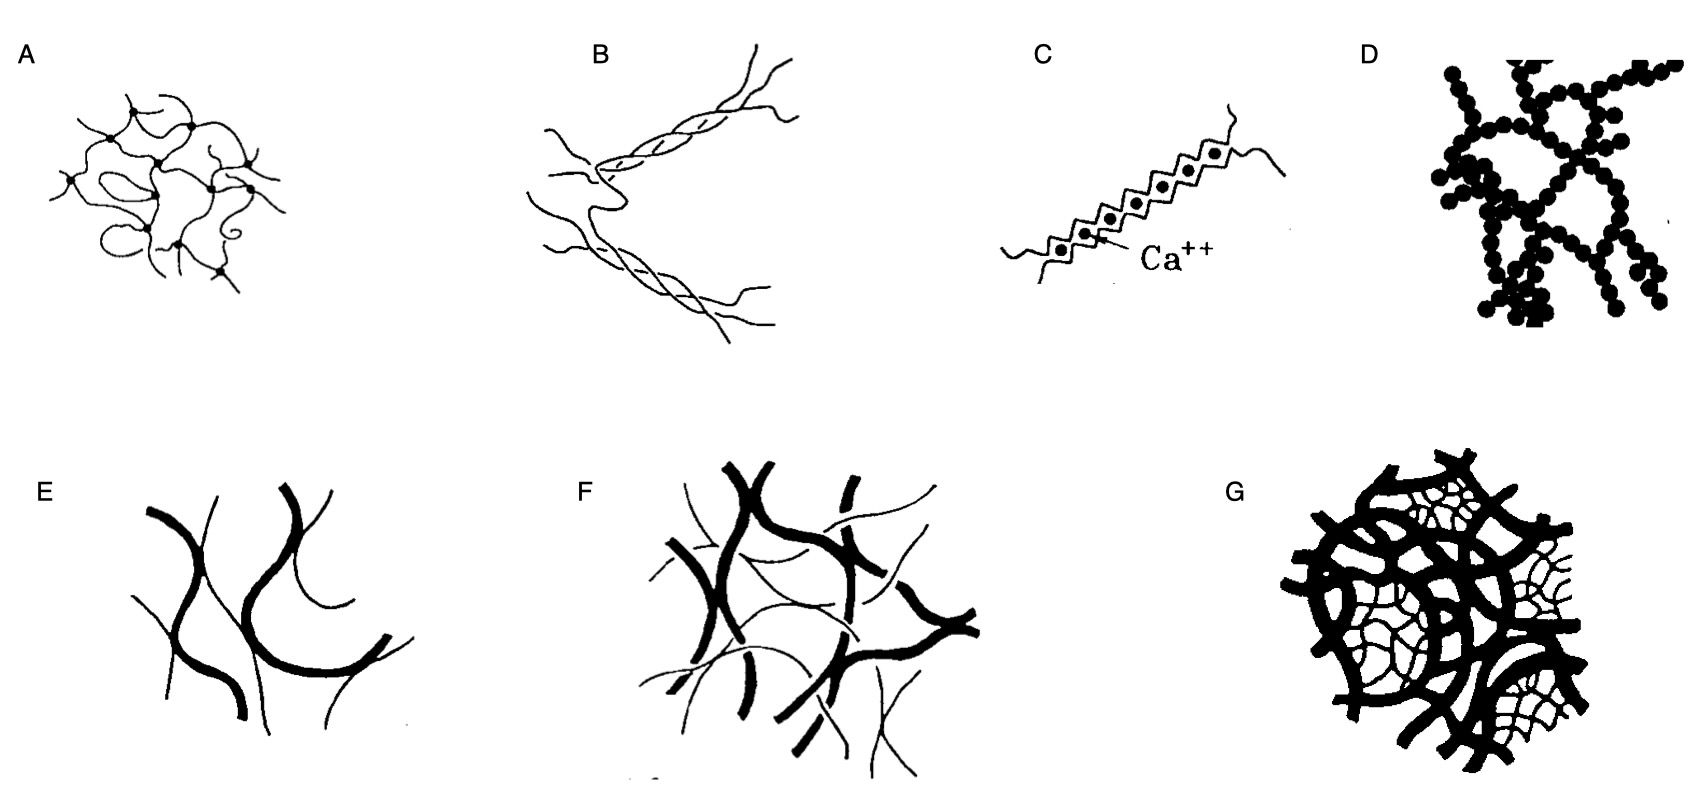
\includegraphics[width=0.8\linewidth]{images/gelation_intro} \caption{Overview of gelation mechanisms, top row displays single component systems, bottow row shows interaction properties of multi component systems:  (A) covalent or chemical gel, (B) thermo-reversible gel, (C) ionic gel, (D) particle gel, (E) coupled networks, (F) inter-penetrating networks, (G) phase separated networks}\label{fig:unnamed-chunk-5}
\end{figure}

Casein gels are not monomeric gels but are formed by interaction of the
four components: alphaS1, alphaS2, beta and kappa casein. When looking
at processed cheese it is evident that it is a composite gel with a
dispersed phase embedded in it. Such systems have been described as
emulsion gels and will be described in the following section.

\subsubsection{Emulsion gels: special types of composite materials}

Process-cheese based casein gels can be viewed as emulsion gels.
Emulsion gels are soft solids with incorporated, emulsified fat droplets
or fat particles. @Dickinson2012 made an intensive description of such
structures which was also based on his own line of research as in
@Dickinson1998, @Dickinson2006. Emulsion gels can incorporate two basic
structures: the emulsion-filled protein gel (A) and the
protein-stabilized emulsion gel (Fig.xx). It should be taken into
consideration, that these two types pose the ideal structure, in real
life models mostly a mix of the two gel types is present at the same
time.

\begin{figure}
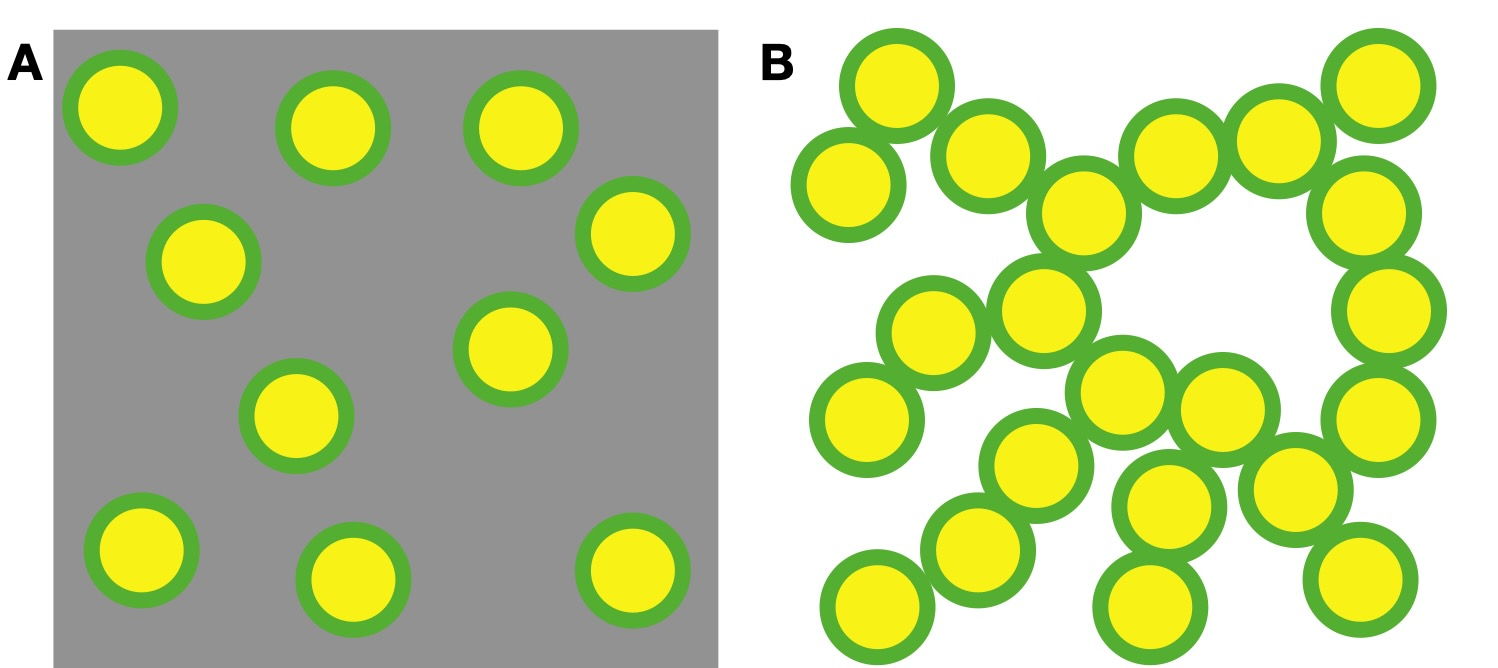
\includegraphics[width=0.5\linewidth]{images/EFG} \caption{Types of emulsion gels: (A) emuslion filled gel, the proteins (green) emuslify the fat (yellow) and are embedded into the matrix; (B) particle gel, the proteins at the interphase connect the fat particles to a continous matrix}\label{fig:unnamed-chunk-6}
\end{figure}

An emulsion-filled protein gel is characterized as a gelled protein
matrix with embedded emulsified fat droplets. The viscoelastic
properties of such gels are mostly determined by the continous phase,
i.e.~the proteins.\\
The protein-stabilized emulsion gel is a type of particulate gel whose
properties are mostly directed by the formation of a network of
aggregated fat droplets, or rather fat particles. The fat particles are
considered filler particles and the properties of the gel are also
directed by the properties of the filler (@Matsumura1993). It was shown,
that gels with incorporated filler in form of fat particles had higher
shear modulii as their fat free counterparts. @Brighenti2018 described
processed cheese as emulsion filled gel. An emulsified fat droplet is
considered to be a solid-like material in both systems. Formation of
emulsion-filled gels usually takes place, when the bulk phase of a
stable emulsion is solidified. Gels of the particulate type are
formulated, when the emulsion droplets aggregate. Destabilization
phenomena in emulsion gels are, for example, induced by excess amounts
of unadsorbed protein that leads to depletion. Another type of
destabilization or stabilization, for the respective matter, is bridging
flocculation (@Semenova2010, @Sapir2015).

\subsection{A complex food system: processed cheese}

In a highly concentrated protein systems, such as processed or cream
cheese, wherein large protein aggregates are present, the inner
structure is usually very complex and influenced by numerous factors.
Furthermore, proteins in biogenic systems generally occur in different
molecular structures as well as molecular scales. Such food systems
often are multi-phased systems. Thus, proteins arise in combination with
other substances, such as fat or carbohydrates. Processed cheese serves
as an example of a complex, highly-concentrated, and multi-phased
protein system. Milk proteins (caseins), fat, and water form a dense
network, triggered by the reaction of caseins with melting salts. The
structure-forming reaction takes place in several stages and only under
certain process conditions. An overview of the general processing steps
and suspected reactions taking place therin is given in Fig.xx.
@Guinee2004 gives an overview of cheese products that are made under
(excessive) heat, meaning they are thermally processed. Such products
are also called pasteurized cheeses. Also, a manufacturing protocol for
processed cheese products is given.

@Fox2016 gives a summary on processed cheese products, additives in
processed cheese and the development of processed cheese throughout the
years. It is mentioned, that heating and shearing of a native cheese
mass leads to coagulation of casein and the release of fat due to the
rupture of the milk fat globule membrane (MFGM) as a result from shear
and heat. Emuslifying salts are used to dsissociate the caseins from
their micellar form, which prevents them from coagulation and leads to
hydration of single caseins that can emulsify the fat phase. According
to the cited literature, the emulsifying salts fulfill the following
functions, or induce them in the caseins:

\begin{itemize}
\tightlist
\item
  upward adjustment buffering of pH
\item
  chelation of calcium after sequestration and de-ionization of the
  micelle calcium
\item
  casein hydration
\item
  binding or emulsification of free fat
\item
  novel structure formation to the processed cheese matrix.
\end{itemize}

The steps necessary to form processed cheese are mainly mixing of the
educts, i.e.~cheese components and subsequent processing of the cheese
mass at Temperatures between 70 - 95 C and constant mixing. The educts
for processed cheese can be in powdered, liguid or in their native,
i.e.~gelled form, when natural cheese is used. Hence the type of mixing
depends on the grain size or dispersity of the primary components or
educts.

Common additives in the production of processed cheeses are whey protein
concentrate, starches or hydrocolloids like carageenaan. These can be
found especially in cream-cheese products, where the dissociation of the
casein micelle is not induced by melting salts, but by acidification. In
such systems, stabilizers in the form of hydrocolloids are often used to
prevent excessive syneresis of the cheeses. Syneresis, the release of
water of gelled dairy systems, is a phenomenon not occuring in processed
cheeses. This might be due to high dry matter, however it is likely,
that the stronger dissociation of caseins into substructures or monomers
(induced by the melting salts) leads to a stronger hydration of the
matrix, since more hydrateable protein units are available in total.

The main component in processed cheese is casein. Their primary
aggregated structure when derived from rennet or native casein gets
disrupted chemically by the melting salts a new structure is build-up
due to the constant shearing and heating of the matrix. The type of
shear applied to the system is in partial determined by the composition
of the educts: when working with fresh cheese curd or (model) cheeses
like mozarella or dried cheese curd, the matrix is more kneaded than
stirred, as it is the case in @Noronha2008, @Noronha2008b,
@Noronha2008c, @Chen2012 and @El-Bakry2001. Processing environments,
where the emphasis was on the investigation of the structure formation
itself at various processing conditions were given, besides others, by
@Cernikova2018a, @Lee2003a, @Guinee2004, @Fu2018, @Fu2018d, @Cunha2013,
@Lenze2019 and in the parallel work of @Vollmer2021. In these studies,
the samples were of a more homogenous or even liquid like sate in the
educt stage and were processed under stirring. A summary of the studies
that dealt with similar systems as in this work can be found at the end
of this section.

\subsubsection{Casein interactions at the presence of melting salts}

Caseins can be described as amphoteric phosphoproteins with different
hydrophobicities (@Horne2017). Their amino acid composition is not
unlike those of globular proteins, however, the high level of proline
hinders caseins to form globular structures. Four different gene
products of caseins can be found not only in bovine milk, the alpha-,
alpha-, beta-, and kappa-casein. The interactions of caseins that lead
to the initial formation of micelles, as well as their interaction
properties in general, have recently been debated (@Horne2017,
@Horne2017b, @Holt2013, @Thorn2015). However there seems to be a common
understanding on two major types of casein interactions that lead to
micelle formation, hydrophobic interactions and the formation of calcium
phosphate nanoclusters (@Lucey2018). Accordingly caseins are molecules
that can interact with each other via hydrophobic interactions,mas well
electrostatic interactions. The casein micelle models presented earlier
in this section are both based on the long established theory that
hydrophobic interactions are a driving force for micelle assembly as
well as casein aggregation (@Horne2017b). Hydrophobic interactions occur
under the exclusion of water. When two opposing surfaces get close, an
energy benefit arises from the new conformation of the water molecules
that were disrupted by the interacting surfaces or structures.

For estimation of the hydrophobicity of caseins, especially in the
special ionic environment present in processed cheese, a hydrophobic
cluster anlysis (HCA) might give further insight (Fig.xx). This type of
computational analysis allows one to take into consideration, that the
caseins are not lacking any kind of substructure, since there is
evidence by the self-association behaviour and the large amounts of
hydrophobic areas in the molecule that the caseins are not intrinsically
unstructured proteins (IUP) (@Huppertz2017, @Lucey2018). Their
flexibility is rather derived from the high amounts of proline that
allow the protein-string of the casein to remain flexible and to not
conform into a globular state. The HCA plots show caseins in a
sub-helical structure with a unit length of \textasciitilde10. The amino
acids in close distance within the plot can form functional areas, such
as hydrophobic clusters. The colouring of the HCA plot is designed to
highlight hydrophobic interaction sites, or clusters. Other amino acids
are highlighted as well. Serin can occur in substituted form (as it is
the case in caseins) as well as threonine, glycine poses a potential
binding site and proline disrupts helical or higher ordered structures.
Therefore, special symbols were chosen, as it is described in
@Rebehmed2016. The plots were created with the website:
\url{http://mobyle.rpbs.univ-paris-diderot.fr/cgi-bin/}
portal.py?form¼HCA\#forms::HCA .

\begin{figure}
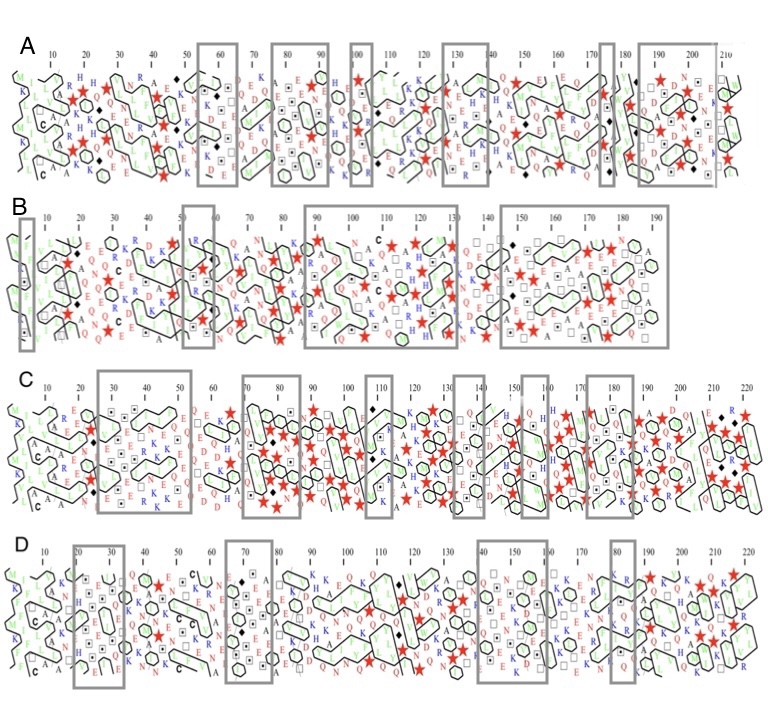
\includegraphics[width=1\linewidth]{images/HCA_serin} \caption{Plots on hydrophobic cluster interactions of caseins:  (A) alphaS1 casein, (B) kappa casein, (C) beta casein, (D) alphaS2 casein; legend as in @Rebehmed2016, with addition of grey squares to highlight serin (dotted square) areas.  hydrophobic amino acids (green) are grouped and surrounded with a solid black line to form clusters, prolin (red star), glycine (diamond), threonine (square) are also highlighted.}\label{fig:unnamed-chunk-7}
\end{figure}

In the HCA plots, caseins comprise of hydrophobic areas that are
disrupted by fractions that carry charge by phosphorylation of serin
(Fig.xx). Serin rich structures were marked (grey boxes), since they are
potential candidates for post-translational transformation, and then
carrying a substituted phosphate group at the serin residue. The charged
areas coming from serine residue display different degrees of
phosphorylation. A direct relationship between the degree of
phosphorylation and calcium binding by chalation has been shown, which
is why the calcium sensitivity of the caseinates is in the order kappa
\textless{} beta \textless{} alphaS1 \textless{} alphaS2. The
distribution of charged serine residues is not uniform in the caseins
(@Aoki1985, @Clare2000). Looking for example at kappa casein
(Fig.xx(B)), it can be seen that the serin residues are arranged over
larger areas in the so plotted molecule, however in little quantities,
when compared to, for example the residues 20-35 in alphaS2 casein (D).
Besides the display of charged residues, the HCA plot also reveals
planar hydrophobic areas, without charge from phosphoserine, due to high
amounts of prolin (indicated by a red star). Such areas can especially
be found in beta casein (see for example amino acids 195 - 120), but
also in kappa casein (amino-acids 60 - 85) and alphaS1 casein (amino
acids 15 - 45). When removing the charge (which means especially
removing the CCP in this case), the planar hydrophobic areas of these
three caseins become even larger. AlphaS2 casein displays smaller planar
hydrophobic areas at amino acids 110 - 120 and 205 - 215. Even more, the
planar hydrophobic area is not increased by removal of the CCP, since
they are not directly neighbouring hydrophobic and proline rich areas in
alphaS2 casein. Hydrophobic interaction happens on the surfaces of the
interacting molecules. Hence the arrangement of planar and hydrophobic
areas in the caseins, with respect to the localization of their serin
rich areas in this arrangement, might give insight towards casein-casein
interaction in the special environment investigated in this work. The
phosphate residues in caseins are relevant in the context of processed
cheese formation, since processed cheese is formed into a new or
``processed'' structure due to the use of melting salts. Melting salts
is a commonly used term for the type of salts that are able to chelate a
divalent calcium cation. Examples for such salts are Mono-, Di- or
Tri-sodiumcitrates, Di- or Tri- Sodium Phosphates, or polyphosphates
like Pentaphosphates or medium chain phosphates, to only cite a few
existing in the context of food and specifically cheesemaking. An
example for a chelated calcium ion by phosphates is given by Fig.xx.

\begin{figure}
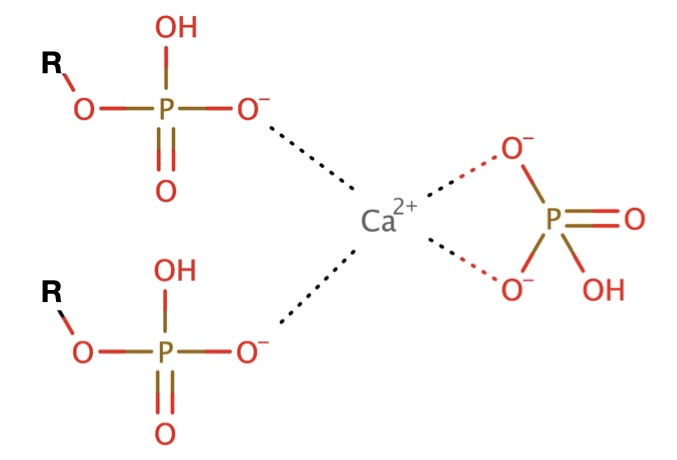
\includegraphics[width=0.3\linewidth]{images/Ca_chelat} \caption{Example of a calcium chelat complex associated with three phosphate groups. R can be either a proteinogenic residue, a calcium phosphate nanocluster (CCP), an associated or bound phosphate, pyrophosphate or polyphosphate or similar.}\label{fig:unnamed-chunk-8}
\end{figure}

The term elusifying salts is used interchangeably with the term melting
salts in this study and elsewhere. However the term emulsifying salt
should not lead to the conclusion, that the salts itself have any
function as emulsifying agents. Rather, as indicated by the term melting
salts, those type of salts lead to a dissociation of CCP in the casein
micelle, which leads to free caseins that can then emulsify a dispersed
phase. The viscoelastic properties however, have proven to be largely
influenced by the type and concentration of emulsifying salts used (See
Tablexx for exemplary studies). It can be suggested, that the chelation
properties in the variety of salts used are not suscepting the CCP all
in the same way, hence the emulsifying salts are mostly used in binary
or ternary mixtures of empirically proven salts.

Since the binding structure of the casein micelle is not yet fully
understood, a conclusive answer on how the emulsification salts work on
the caseins or casein micelles, respectively, cannot be given. The
chelating salts enter the casein micelle during hydration through
microfluidic channels. To a certain extent, also strongly depending on
the type of salt used, the calcium from the CCP gets released, a
shrinkage of the micelle and also the release of single caseins was
reported at low concentrations, at higher concentrations, complete
dissociation of the micelle took place. However, various studies showed
the different behaviour of a casein matrix, depending on the type of
salt used (@Sadlikova2010, @Salek2017, @Awad2002, @Salek2015b,
@Brickley2008, @Chen2012, @Nagyova2014 and others). An observation made
in the cited works was that ideal ratios of emulsifying salts can target
special properties of the final product, such as hardness or
spreadability. In general, a higher amount of phosphate salts resulted
in higher viscosities or hardnesses of cheeses. The best products were
given, when not one salt, but a ternary mixture of emulsifying salts was
present, ideally combining a polyphosphate, a di- or tri-phosphate and a
citrate.

A detailed analysis of the structures of model processed chesses similar
in composition to this matrix were investigated containing different
amounts of Polyphosphates next to the other emulsifying salts, also used
herein (@Vollmer2021a). The samples were analyzed using transmission
electron microscopic (TEM) imaging, elucidating the structures on a nano
scale. An effective increase in cheese hardness could be found with
increasing amounts of polyphosphate. Also a threshold value of 1.5\% of
polyphosphate was necessary to induce the creaming reaction. A detailed
description, what leads to the formation of casein fibrils in other
environmens can be found in the cited work. Other interactions of
caseins in an environment containing melting salts are of elctrostatic
or general hydrophilic nature.

\subsubsection{The Creaming Reaction}

The development of processed cheese took place around the beginning of
the 20th century. The aim at that time was to develop a method to extend
the shelf life of cheese and thus to store it longer and also to be able
to export it. In 1911, the Swiss inventors W. Gerber and F. Stettler
succeeded in transforming raw cheese into a homogeneous, flowable state
through the application of sodium citrate as a melting salt. From this
``sol'' state, a solid, homogeneous ``gel'' formed again after cooling.
At the same time, a processed cheese based on cheddar cheese was also
developed in the USA. Here, citrates and orthophosphates were already
used as melting salts. In 1917, the KRAFT company launched the first
processed cheddar cheese on the market, which was initially intended for
army rations. The company Gebrüder Wiedemann from Wangen in Allgäu did
not conquer the European market until 1921.

Initially, the grinded cheese, cheese mass or protein-fat-mixture, is
mixed with melting salts and then heated under constant shear. In this
melting phase, the calcium is chelated by the melting salts and replaced
by sodium. This results in a dispersion of the casein, which
increasingly dissociates due to the lack of calcium phosphate bridges
and binds the fat into the protein network. Emulsifying salts generally
increase the stability of cheese emulsions under thermal treatment
(@Hougaard2015). During the production of processed cheese, first a
gel-sol transition and then again a sol-gel transition takes place. The
transformation from insoluble gel to sol takes place through the
application of heat and mechanical processing. This process works in
processed cheese, in contrast to normal cheese, where only a phase
separation would occur, through the addition of melting salts. The salts
add effective charge carriers to the system, the calcium is removed from
the casein by ion exchange, and the polypeptide chains bind water,
resulting in swelling of the matrix. The subsequent sol-gel transition,
in which the flowable mass becomes a solid cheese again, is achieved by
subsequent cooling. Accordingly, the ``creaming reaction'' is an ion
exchange reaction in which the gelatinous cheese structure is converted
into an emulsion with a spreadable structure under the action of energy
and melting salts. The subsequent structure build-up after melting,
during which complex physicochemical reactions take place, is called
post-creaming. If the structure loses its spreadability as a result of
too long post-creaming, this is referred to as overcreaming of the
processed cheese, which results not only in very solid gel formation but
also in the escape of fat and water (@Lenze2019).

@Vollmer2021 suggested to update the term ``creaming'' or ``creaming
reaction'' to the term ``texturizing''. The term creaming can be
misinterpreted in this context, since it is also used for the
description of emulsion instability: when the fat phase, especially in
milk (fat) or cream protrudes to the surface of the emulsion, the
emulsion is said to be ``creamed''. The term texturization would fit the
process in a better way, since texturizing, i.e.~the aggregation of
caseins in some kind, leads to the formation of the desired structure.
The properties of the final product are seemingly effected more by the
composition of the matrix than the processing conditions. Hence a more
spreadable product will be rather obtained by the use of more water and
or fat, than shorter processing times or lower processing temperatures
or speeds.

\subsection{Investigation of process parameters and composition on the structure formation during manufacture of processed cheese}

The final structure of the processed cheese depends on the starting
material as well as the processing conditions. Various studies have been
performed analyzing the effects of matrix composition and processing
conditions on the final texture of the cheese matrix. @Fu2018
investigated different emulsification conditions for their influence on
the microstructure of a model cheese network. Stirring speeds of 400 rpm
and 1500 rpm, and process times of 10 min and 30 min were varied. The
microstructure of the resulting protein network was identified by SEM,
and the distribution of the fat globules by CLSM. Regardless of the
stirring speed, a so-called ``fine-stranded-network'', i.e.~a network of
protein (aggregates) arranged together like fibers, was shown here after
30 min. In addition, a start-up phase, as well as an exponential phase,
was recognizable during the processing of the matrix of 30 min. However,
longer processing times were not targeted here to identify the full
course of protein aggregation.

\textbf{Bild Grafik der verschiedenen Netwerke machen}

This work also dealt with the effect of rework, i.e.~already
pre-processed processed cheese mass added to the raw materials at the
beginning of the reaction, and its effects on the structure formation.
It was shown that only sufficiently processed mass can ensure
acceleration of network formation. The effect of the rework is
manifested by smaller fat globules and a finer, more ordered network in
the final product. However, no mechanistic explanation of the processes
is provided, but only the phenomenon or the effect of rework on the
final product is described. @Cernikova2018a also studied the effect of
rework at different concentrations (0 - 20\% of dry matter). Again,
smaller fat globules as well as a fine, fibrous network and increasing
hardness of the final product were observed up to a rework concentration
of 10\%. When the rework concentration was increased further, no
significant change in the final product was observed. Although this work
provides a good overview of compositional and process-related effects of
rework addition, it does not provide a mechanistic explanation.
@Lenze2019 investigated a process cheese matrix and the effects of
rework addition. Processing time was significantly reduced under rework
addition. This effect was explained by an autocatlytic effect.
Favourably aggregated proteins act, similar to a seeding effect in
crystal systems, as a template which leads to structuring the other
proteins in the system in the same way. From this, it could be concluded
that proteins or proteinogenic systems structurally similar to caseins
aggregate within a certain process environment to form hydrophobic
clusters and then eventually to a large network stabilized via
hydrophobic interactions. @Guinee2004 also dealt with similar systems.
Here, structure formation was interpreted as a consequence of hydration
of proteins and as a consequence of increasing viscosity during cooling
of the hot mass.

A possible cause of the viscosity increase was overall described as
exposure to the ionic environment with the effect of complexation of
stabilizing calcium ions results in dissolution of the casein micelle,
exposing the hydrophilic and hydrophobic sections of the individual
caseins. Consequently, hydration of caseins occurred due to hydrophilic
interactions with the aqueous phase and interactions of caseins with the
fatty phase via hydrophobic interactions. These interactions also led to
emulsification of the fatty phase.

@Cunha2013 showed the influence of different fats (soybean oil,
partially hydrogenated soybean oil and milk fat in the form of butter)
on the rheological, functional and sensory properties of spreadable
processed cheese analogs. Smaller fat globules were observed in
unhydrogenated fats, which was explained by the greater steric
inhibition of unsaturated fatty acids and resulting therfrom, lower
hydrophobic interactions among fat molecules. In addition,
unhydrogenated, or unsaturated, fats have a lower viscosity, which makes
the fat easier to break down during processing. @Soowiej2014
investigated the effect of inulin as a fat-replacement in processed
cheese. @Ramel2018 gave a protocol for the replacement of milk fat with
canola oil in analogue cheeses and also used oat fiber particles for
better stabilization. Other additives, such as starches were
investigated in the works of @Noronha2008b. As already mentioned
earlier, excessive studies have been performed on the effect of
different amounts and types of emulsifying salts. Concluding this
section, it can be stated that processed cheese is a vastly investigated
model system. The focus was predominantly on the effects of processing
or compositional changes on the final product. Only few studies have
performed that followed the structure buil-up in a targeted manner.
@El-Bakry2011 and @Noronha2008c investigated multiple samples during the
formation of a processed cheese mass. However, since the samples were
largely inhomogenous, the different stages of structure formation could
be identified but not followed in an analytical way.

\subsection{Compositional analysis of model processed cheese systems}

Model processed cheese systems have been investigated widely in
macroscopic terms, as described previously in this section. A
compositional anlysis can be defined as an analysis not just in the
makrostructure represented as viscosity, gel strength or any of the
such. In addition, a compositional analysis cannot be given conclusively
by imaging techniques, since the electron density of the casein
particles is too similar.

Spectroscopic measurements like Fourier Transform Infrared (FTIR)
spectroscopy gives insight towards the intermolecular binding in
molecular, giving general conclusions towards the structure of
molecules. It is best applied to rather dry or powdery samples and was
used for example for the structure determinition of processed cheese
made with additives like starches, as it was done in @Noronha2008b. FTIR
proved to be useful to elucidate such structures in the matrix, that are
of distinctly different composition. For structure elucidation of very
similar but differently aggregated casein structures, FTIR is not the
proper tool since the differences in aggregation are too small in terms
of their possible excitation state by IR.

For a compositional analysis of fat-free protein mixtures, native or
reducing SDS page is a commonly used method. An SDS page is a type of
polyacrylamid gel-electrophoresis (page), where Sodium Dodecyl Sulfate
(SDS) is used to charge the protein residues nagtively and then
separating them by size using a strong electric field. The term
``native'' in this context means, that no reducing (as respective for
the treatment) agent like Dithiotreitol (DTT) was used in the samples.
DTT leads to the disruption of Dithio- or Thiol induced bonds or
interactions.

Another method to determine the protein concentration in dense matrices
is the method by Dumas, where the sample is burned and the total
released nitrogen from this process is measured and calculated to a
protein concentration, using an empiric factor. As already indicated
when describing the SDS procedure, the determination of protein
concentration after the method of Dumas also requires almost fat free
samples, since the samples are burned and too much fat would lead to the
disruption of the mesuement due too the bruning of the fat phase.
Analysis by SDS page also is not suitable for processed cheese samples,
since the SDS will, as a tenside, also bind to the fat-phase and
therefore, clear protein bonds are not visible in fatty systems. This
effect is known to the person skilled in the art and is due to the
overlay or ``smearing'' of the fat in the runs. To determine the
structuring mechanisms in processed cheese however on a molecular level,
a compositional analysis seems urgently necessary. Therefore a
compositional analysis herein is a description of either the
distribution (\%) or concentration of certain molecular components
within the matrix.

\subsubsection{Analysis by reversed phase chromatography}

Reversed phase high-pressure liguid chromatography (RP-HPLC) is a
technique widely used in compositional analysis, especially in food
systems. In food analysis, quick and easy measures for Quality Assurance
can be implemented, as well as detailed compositional analysis of food
matrices up to Liquid Chromatography in general uses a statinary phase
and a moblie phase with respective opposite polarities. Besides polar or
apolar columns, a magnitude of other columns are available, reaching
from columns with a special pore size for size exclusion chromatography
or ionic columns for respective ion analysis in terms of
ion-exchange-chromatography. The detector unit when investigating
proteinogenic materials is usally a diod array detector (DAD), with
detection in the UV-Vis. for proteins, a detection is usually made
around a wavelength of 280 nm, since the aromatic amino acids get
excited in the UV. This requires, of course, the use of pure standards
for calibration, since the excitation of individual proteins in the UV
is specific and different for every species.

The basic principle of a rephersed-phase chromatography experiment is
the use of a hydrophobically substituded, i.e.~a non-polar or
reversed-phase, silica gel as the chromatographic column. As already
mentioned, the column represents the stationary phase, whereas the
sovent or eluent represents the mobile phase, which transports the
analytes to and through the column. For RP\_HPLC this means, that the
mobile phase is of rather polar nature. In RP-HPLC experiments,
specifically designed to target dairy proteins, the mobile phase used is
usually used as gradient elution. Gradient elution means, that the
polarity of the mobile phase is adjusted (either gradually or step-wise)
during the measurement, to better elute the sample components from the
column. @Bonfatti2008 first showed a measurement for the simultaneous
measurement of caseins next to whey proteins. The buffer system most
suitable for this type of measurement was presented by @Bonizzi2009 and
is described in chapter 4 of this work. @Dumpler2017 was able to reduce
the experiment length significantly by improving the elution of whey
proteins next to caseins from the column. The chromatogramm which is
obtained by that process as well as the identification of the elutes is
shown in Fig.xx.

\begin{figure}
\centering
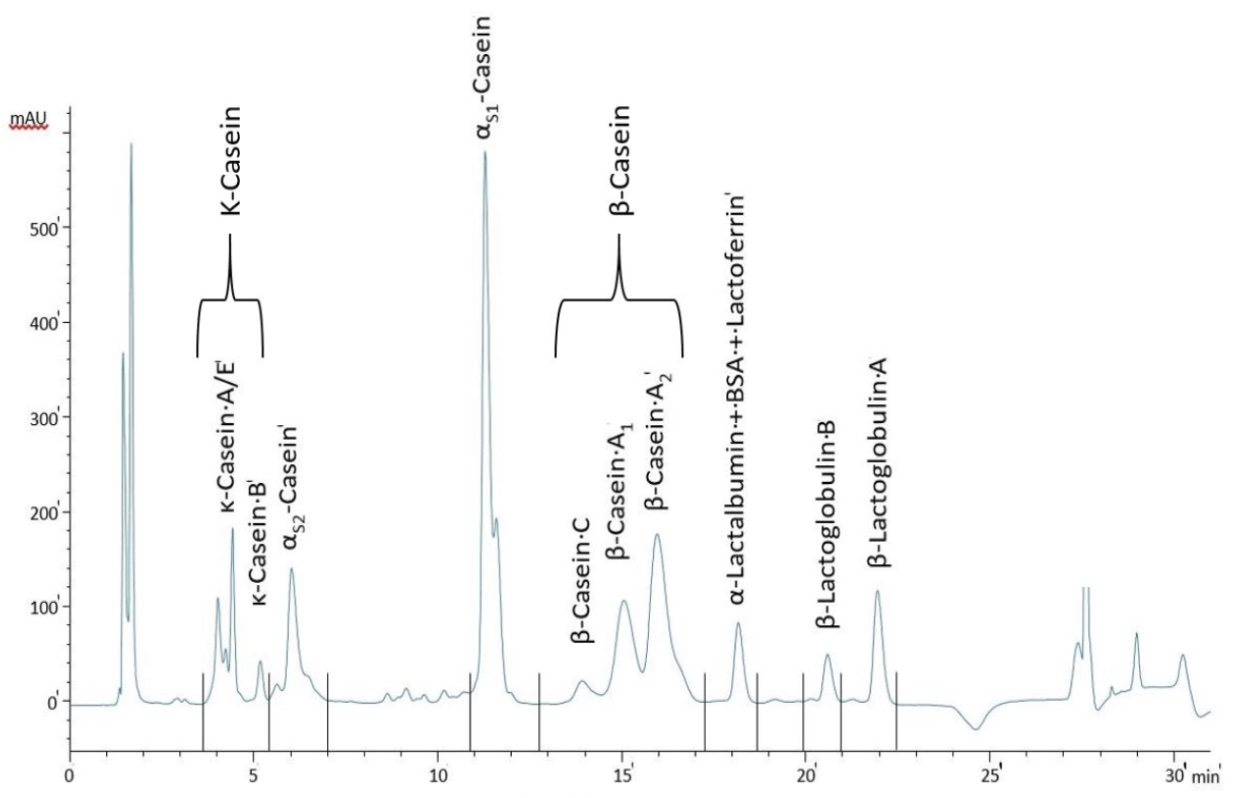
\includegraphics{images/elution_casein.jpg}
\caption{Casein elution in RP-HPLC after @Dumpler2018, next to whey
protein elution}
\end{figure}

It has been shown, that RP-HPLC is a powerful tool for protein
quantification. However, as already discussed in the beginning of this
section, fat-rich samples pose to be a problem as well. The isolation of
caseins from the fat phase seems crucial in order to determine the
functional properties of the dispersed phase in the system.

\subsubsection{Investigation of 1H T2 relaxation}

The measurement of longitudinal relaxation of protons aver being excited
by a magnetic spin is a readily used technique for compositional
analysis. The principle of those type of measurements lies in the fact
that positive nucleii have a magnetic spin. This spin can be exited
using a polarized magnetic field. By the use of a spin-echo-train,
better known as CPMG sequence, a pulsed magnetic field puts the spins
back into the direction of the magnetization vector, but with a decaying
intensity due to the interaction of the spins with the surrounding
matrix. The CPMG sequence is especially useful when applied in dense
systems (@Schmidt2004, as in @Hinrichs2007). A more detailed description
of the principles underlying the NMR T2 relaxation measurement is given
by Fig.xx.

\textbf{Figure} of how data is obtained during the NMR measurements with
CPMG sequence

Some of the composite model systems already described herein were also
investigated using T2 relaxation times. In the following section, the
systems most similar in their experimental approach or composition are
described below in more detail.

In @Chen2012, a matrix consisting of differently ripened mozarella as
the protein source and butter as the fat phase was processed to a
coherent cheese matrix and anlyzed using T2 relaxometry. The components
were fitted using the LaPlace inversion computer program, further
details of the fitting process were not disclosed. Four components were
fitted, however instead of attributing one of the fittet peaks in the
distribution to the fat phase as done elsewhere, the two peaks between 1
and 100 ms were attributed to water, with no further explanation as to
why. @Noronha2008c investigated an imitation cheese matrix made from
particulate rennet casein, vegetable oil emulsifying salts and 53\%
water, processed in a Farinograph cooker. The matrix was constantly
kneaded and analyzed, \emph{inter alia}, in their T2 relaxation times.
The middle component was attributed to the fat fraction. @El-Bakry2011
investigated a model processed cheese system, prpared with a
Farinograph-type cooker, in order to follow the structure build-up
during processing. Samples with a lowered amount of emulsifying salts
were also tested. The T2 relaxation times proved a lesser casein
hydration and a longer time for fat emulsification in an environment
with reduced amounts of melting salts.

\subsection{Studies related to this work}

The studies performed by @Roeck2010, @Lenze2019 and @Vollmer2021,
@Vollmer2021a are in direct relation to this work, since an equal model
processed cheese composition as it was in this study was investigated.
@Lenze2019 (or @Roeck2010, respectively) did a vast investigation and
characterization of a model processed cheese mass that was processed
(constant heating, constant stirring) in a rheometer as a processing
device. The rheometer was set-up with a custom made cup and a two blade
stirring rod in order to make use of both of its functions; as heating
and shearing - in our case stirring - device as well as instrument to
detect changes in the Torque of the stirrer, which was interpreted as
apparent viscosity during this process. A step-wise structure formation
process was reported, and the processed matrix was roughly characterized
at distinct processing times, using imaging techniques (LM, TEM). The
process parameters influencing the structure formation of the model
matrix were investigated. An analysis by comparison was performed,
investigating the influence of variances in model composition on the
detected structure formation. A summary of the investigatted parameters
(process and ``compositional'') is given in Tablexx. From the obtained
data, the step-wise structure formation process could be characterized
into the following phases:

\begin{enumerate}
\def\labelenumi{(\alph{enumi})}
\tightlist
\item
  an initial phase (0 - 25 min), where matrix hydration and therefore
  chemical reactions take place,
\item
  a first exponential phase (25 - 140 min), characterized as an increase
  in apparent viscosity, dedicated to the formation of a stable emulsion
  in the system, up to a\\
\item
  plateau phase (140 - 180 min), characterized as de-emulsification,
  concluded by
\item
  a second exponential phase (180 - 225 min), characterized as protein
  network formation.
\end{enumerate}

The formed structures were characterized on a microscopic level by fat
globule size and light imaging, on the macroscopic level by oscillatory
shear rheology. Values for pH and dry matter of the products were
obtained. Besides sampling for LM imaging, the process was investigated
as a whole. No explanations on a molecular, i.e.~casein-casein
interactions concerning level were made.

\begin{longtable}[]{@{}
  >{\raggedright\arraybackslash}p{(\columnwidth - 2\tabcolsep) * \real{0.05}}
  >{\raggedright\arraybackslash}p{(\columnwidth - 2\tabcolsep) * \real{0.95}}@{}}
\caption{parameters influencing the structure formation of model
processed cheese}\tabularnewline
\toprule
Investigated parameter & Key results \\
\midrule
\endfirsthead
\toprule
Investigated parameter & Key results \\
\midrule
\endhead
Stirring speed & Higher processing speed lead to weaker gels due to a
proposed structure corruption from the applied shear \\
Temperature & ≥ 70°C necessary to initiate creaming reaction \\
Protein composition & Model matrix was derived from natural cheese with
addition of 2\% (w/w protein) protein powder of varying sources).
Presence of whey proteins, native casein and rennet casein promotes the
occurrence of a distinct first exponential phase, whereas acid casein
and sodium caseinate lead to absence of a first exponential phase but
show a pronounced exponential increase in apparent viscosity at late
processing times \\
Protein concentration & Higher concentration in proteins results in
stronger gels and stronger display of a step-wise structure buil-up \\
Addition of rework & Highly accelerated structure formation, values of
5\% and 10\% were investigated, higher rework concentration also leads
to even faster structure formation \\
pH educt & Optimum pH for the creaming reaction to occur in this set-up:
5.83 - 5.96 \\
Fat globule size & Smaller Fat globules accelerated structure
formation \\
Fat composition & Use of surface active ingredient in systems made from
oil as the fat phase strongly accelerated structure formation;
\emph{Note: model for the present study was chosen from this data set
and was the control (oil, no emulsifier, with Lactose as dry matter
add-on), but used without Lactose during this trial.} \\
Fat concentration & Presence of fat is needed to display step-wise
structure formation; very low structure formation without presence of
fat; Lactose was used as dry-matter add on in samples with reduced fat
content \\
\bottomrule
\end{longtable}

@Vollmer2021 investigated the same model processed cheese mass that was
investigated in this study, but with adapted process parameters to give
a long processing time (total of 415 minutes). The processing of the
samples, followed a sampling procedure that is key to this study, and
will be presented later on. This allowed, to give six consecutive
samples to be investigated by LM imaging and TEM imaging. The obtained
images strongly suggested the formation of casein fibrils. In fact, it
was suggested, that the casein fibrils were prominent for the structure
formation reaction, that is the ``creaming''-reaction. An updated model
for the proposed structure formation processes that take place in
processed cheese is displayed in Fig.xx.

\begin{figure}
\centering
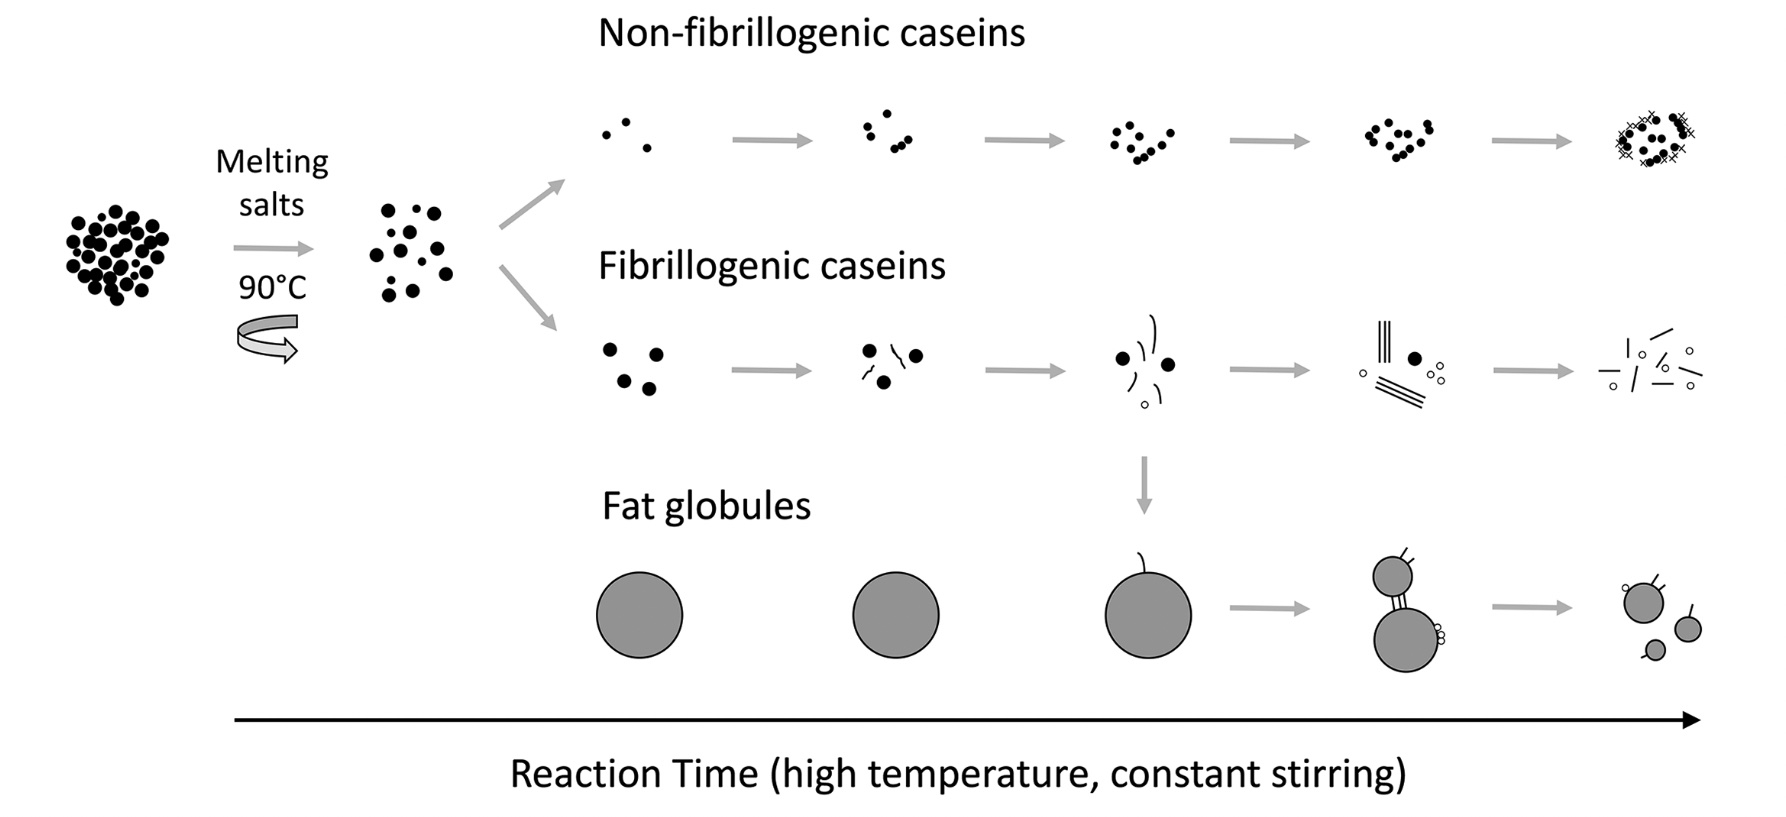
\includegraphics{images/str.form_Vollmer.jpg}
\caption{Model presented for structure formation reaction as cited in
the literature; formation of fibrillogenic caseins and non-fibrillogenic
caseins; fibrillogenic caseins emulsify the dispersed phase and later
seem to form a particulate network}
\end{figure}

The obtained TEM images showed the formation of large entangeled or
interconnected networks with fibrillar structure. During the plateau
phase of the structure formation, elongation of the detected fibrils was
apparent. The emulsification of the fat was considered mainly due to
specific interactions of the fibrillar structures with the fat phase.
Even more, the followed structure build-up revealed the progressive
separation of the casein matrix, into protein dense, fibrillary
aggregated areas and areas with low protein density. At late stages of
processing, degradation of the fibrils becomes evident. @Vollmer2021a
investigated a model processed cheese matrix that had varying amounts of
a binary mixture of emulsifying salt. The samples were processed in the
same manner as above. Casein fibrils were present at later processing
times, also the progressive phase separation already beginning at early
stages of processing in @Vollmer2021 could be seen at later processing
stages. An important threshold value for this study could be given: the
degree of dissociation of the casein micelle in the model system,
measured as the amount of insoluble calcium after acid-base titration
depends on the concentration of a specific emulsifying salt. A
compositional analysis was made to investigate the fibrils, which were
detected as a slight increase of kappa casein in the insoluble pellet
after ultracentrifugation.

@Lee2003a gave a model description (Fig.xx) for the formation of a
protein matrix in processed cheese. It was indicated, that the casein
monomers form a string like network, not unlike a particle gel, which
resulted in a peak in viscosity.

\begin{figure}
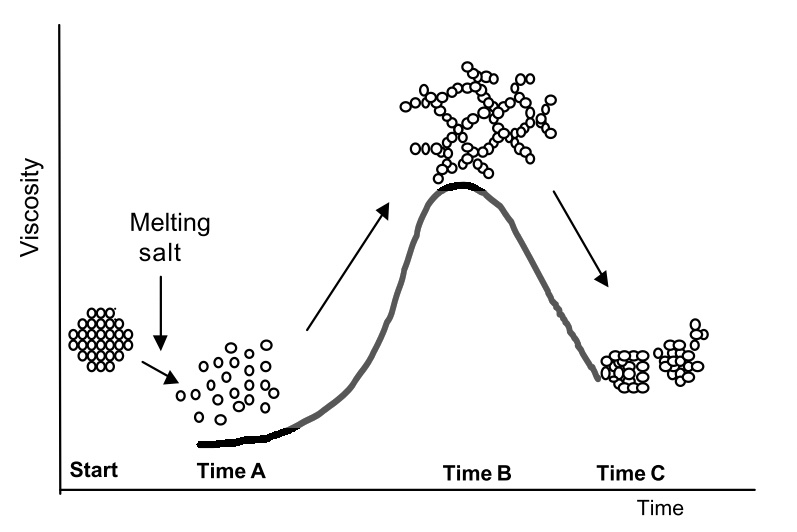
\includegraphics[width=0.5\linewidth]{images/str.frm_Lee} \caption{Structure formation and destruction process as indicated by viscosity of a fat-free processed chess mass as cited in the literature; Protein network formation leads to a peak in viscosity, in a fat free formulation the collapse of the network is visible by decreasing viscosity}\label{fig:unnamed-chunk-13}
\end{figure}

From comparison to a fat-free model, it was concluded that the connected
protein matrix collapses to form dense units. It was concluded that fat
was not prevalent for the creaming reaction to occur and emphasized
protein protein interactions. The industrial terms for typical errors in
processed cheese, namely ``undercreamed'', ``creamed'' and
``overcreamed'' were brought into context with the observed structure
formation and structure destruction processes. To conclude this section,
Tablexx gives a summary of recent works already cited in this section,
due to likewise protein matrices.

\begin{longtable}[]{@{}
  >{\raggedright\arraybackslash}p{(\columnwidth - 2\tabcolsep) * \real{0.10}}
  >{\raggedright\arraybackslash}p{(\columnwidth - 2\tabcolsep) * \real{0.90}}@{}}
\caption{Studies on processed cheese relevant for this
work}\tabularnewline
\toprule
Author(s) & Investigation/Key findings \\
\midrule
\endfirsthead
\toprule
Author(s) & Investigation/Key findings \\
\midrule
\endhead
@Brighenti2018 & Acid induced cream cheese and the effect of low or high
pressure (HP) pre-treatment and fermentation temperature (FT) by means
of Rheology and numeric analysis \\
@Berta2016 & Small amplitude oscillatory shear rheology of natural
cheese compared imitation (i.e.~processed cheese) in conditions relevant
for baking \\
Sadlikova et al.~(2010) & Effects of Phosphate salts on the viscoelastic
properties of processed cheese, tested with oscillation rheology; \\
@Salek2015b, Salek et al.~(2017) & Textural and viscoelastic properties
of spreadable model processed cheese (dM = 35\%, fat in dM 50\%) as
effected by mixtures of the following melting salts: disodium
hydrogenphosphate (DSP), tetrasodium diphosphate (TSPP), medium chain
(n=20) polyphosphate (PP), trisodium citrate (TSC). Hardest cheese was
found in 1:1 mixtures of DSP and TSPP. Effects of storage time was also
investigated \\
@Awad2002 & Different ratios of emulsifying salt mixtures and their
effect on adhesiveness and hardness during storage. \\
@Brickley2008 & Effect of emulsifying salts and special ratios on
non-fat processed cheese, samples from TSC as emulsifying salt showed
higher creaminess and lower pH \\
@Hougaard2015 & Stability of hot processed cheese mass improved by
addition of emulsifying salts during holding \\
@Chen2012 & Increase of pH, hardness and casein dissociation with higher
amounts of emulsifying salts are reported. \\
@Guinee2004 & Overview of pasteurised or processed cheese products in
terms of preparation, composition and properties \\
@Cunha2013 & Effects of different types of fat (butter, plant oils and
hydrated plant fat) in spreadable cheese analogues on mainly
viscoelastic properties and consumer acceptance \\
@Soowiej2014 & Fat replacement with inulin in model processed cheeses
with added whey proteins resulted in higher cheese hardness and lower
meltability \\
@Cernikova2018a & Effects of the addition of rework (i.e.~pre-processed
cheese) from 2.5 -10\% on the viscoelastic properties of processed
cheeses, increased firmness was reported due to rework addition, amounts
exceeding 10\% had no further effect \\
@El-Bakry2011 & Casein hydration and fat emulsification investigated
during processing, also with the influence of emulsifying salt reduction
(resulted in weaker gels) \\
Noronha et al.~(2008(1), 2008(2), 2008(3)) & Textural properties, effect
of additives monitored parameters were the hydration of the casein
matrix and the emulsification of fat as investigated by T2 relaxation
NMR, FTIR and texture analysis methods; Samples were taken during
processing. \\
@Ramel2018 & Replacement of milk fat with canola oil to increase
nutritional value of analogue cheese; addition of oat fibres for better
product stability \\
@Sharma2016 & Model mozzarella cheeses and the effect of different
amounts of shear work input; non-linear increase in apparent viscosity
with increasing shear work input (i.e.~kneading). \\
@Lee2003a & Ground work for many subsequent study like this one, step
wise structure formation reported as well as its independence from the
presence of fat \\
@Gogaev2009 & Analysis of varying amounts of protein and fat
concentrations on the microstructure of processed cheeses \\
Nagyova et al.~(2014) & Effect of ternary mixtures of emulsifying salts
on viscoelastic properties. \\
@Barth2017 & Effect of pH and polyphosphate on the cheese structure,
measured with 31P nuclear magnetic resonance technique \\
@Kosfa2018 & Effect of fat and emulsifying salt reduction on
physicochemical properties of white brined cheese emulsions; apparent
viscosity with pseudo plastic flow behaviour increased with fat
reduction; essentially a degree of emulsifying salt concentration is
necessary to form a stable emulsion without effects of creaming or
clustering. \\
@Vogt2015 & Dissfusing wave spectrometry (DWS) and small amplitude
oscillation rheology performed on heated cheeses (Mozzarella, medium
Cheddar, aged Cheddar), progressive increase of free water in the system
as cheese is heated. \\
@Fox2016 & Fundamental principles on cheese, recent review on processed
or imitation cheese matrices \\
\bottomrule
\end{longtable}

\end{document}
